%\documentclass{standalone}
%\usepackage{tikz}
%\usetikzlibrary{patterns,plotmarks}
%\begin{document}
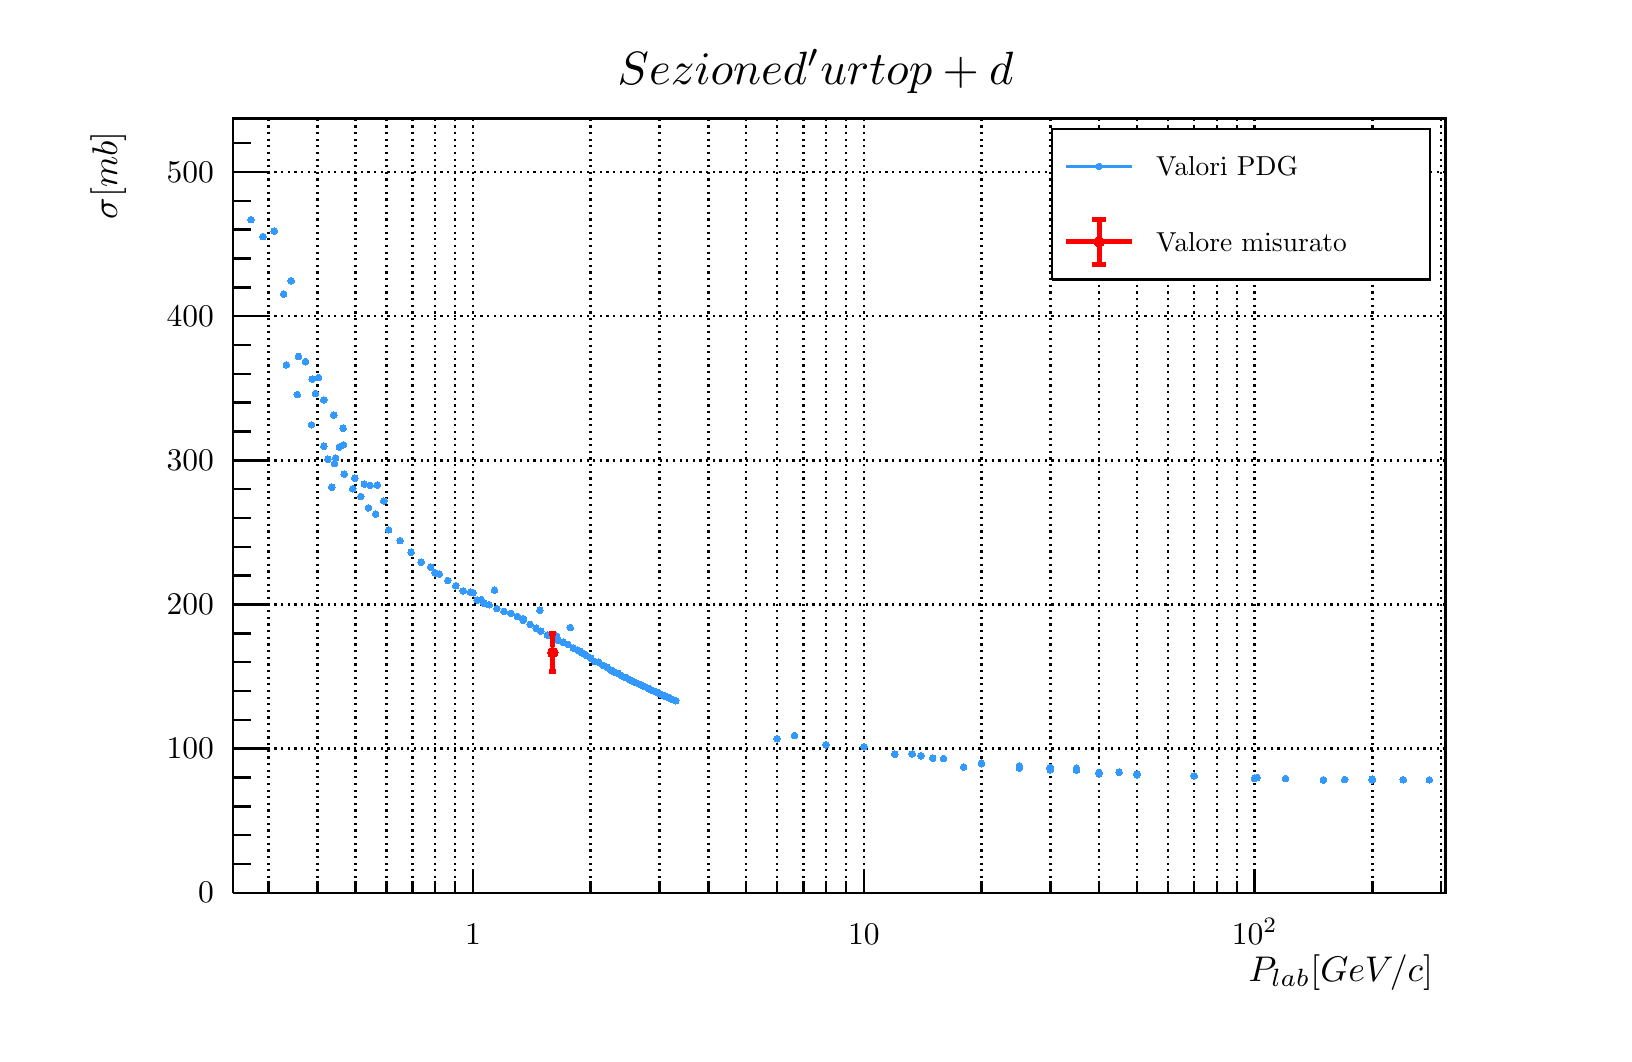
\begin{tikzpicture}
\def\CheckTikzLibraryLoaded#1{ \ifcsname tikz@library@#1@loaded\endcsname \else \PackageWarning{tikz}{usetikzlibrary{#1} is missing in the preamble.} \fi }
\CheckTikzLibraryLoaded{patterns}
\CheckTikzLibraryLoaded{plotmarks}
\pgfdeclareplotmark{cross} {
\pgfpathmoveto{\pgfpoint{-0.3\pgfplotmarksize}{\pgfplotmarksize}}
\pgfpathlineto{\pgfpoint{+0.3\pgfplotmarksize}{\pgfplotmarksize}}
\pgfpathlineto{\pgfpoint{+0.3\pgfplotmarksize}{0.3\pgfplotmarksize}}
\pgfpathlineto{\pgfpoint{+1\pgfplotmarksize}{0.3\pgfplotmarksize}}
\pgfpathlineto{\pgfpoint{+1\pgfplotmarksize}{-0.3\pgfplotmarksize}}
\pgfpathlineto{\pgfpoint{+0.3\pgfplotmarksize}{-0.3\pgfplotmarksize}}
\pgfpathlineto{\pgfpoint{+0.3\pgfplotmarksize}{-1.\pgfplotmarksize}}
\pgfpathlineto{\pgfpoint{-0.3\pgfplotmarksize}{-1.\pgfplotmarksize}}
\pgfpathlineto{\pgfpoint{-0.3\pgfplotmarksize}{-0.3\pgfplotmarksize}}
\pgfpathlineto{\pgfpoint{-1.\pgfplotmarksize}{-0.3\pgfplotmarksize}}
\pgfpathlineto{\pgfpoint{-1.\pgfplotmarksize}{0.3\pgfplotmarksize}}
\pgfpathlineto{\pgfpoint{-0.3\pgfplotmarksize}{0.3\pgfplotmarksize}}
\pgfpathclose
\pgfusepathqstroke
}
\pgfdeclareplotmark{cross*} {
\pgfpathmoveto{\pgfpoint{-0.3\pgfplotmarksize}{\pgfplotmarksize}}
\pgfpathlineto{\pgfpoint{+0.3\pgfplotmarksize}{\pgfplotmarksize}}
\pgfpathlineto{\pgfpoint{+0.3\pgfplotmarksize}{0.3\pgfplotmarksize}}
\pgfpathlineto{\pgfpoint{+1\pgfplotmarksize}{0.3\pgfplotmarksize}}
\pgfpathlineto{\pgfpoint{+1\pgfplotmarksize}{-0.3\pgfplotmarksize}}
\pgfpathlineto{\pgfpoint{+0.3\pgfplotmarksize}{-0.3\pgfplotmarksize}}
\pgfpathlineto{\pgfpoint{+0.3\pgfplotmarksize}{-1.\pgfplotmarksize}}
\pgfpathlineto{\pgfpoint{-0.3\pgfplotmarksize}{-1.\pgfplotmarksize}}
\pgfpathlineto{\pgfpoint{-0.3\pgfplotmarksize}{-0.3\pgfplotmarksize}}
\pgfpathlineto{\pgfpoint{-1.\pgfplotmarksize}{-0.3\pgfplotmarksize}}
\pgfpathlineto{\pgfpoint{-1.\pgfplotmarksize}{0.3\pgfplotmarksize}}
\pgfpathlineto{\pgfpoint{-0.3\pgfplotmarksize}{0.3\pgfplotmarksize}}
\pgfpathclose
\pgfusepathqfillstroke
}
\pgfdeclareplotmark{newstar} {
\pgfpathmoveto{\pgfqpoint{0pt}{\pgfplotmarksize}}
\pgfpathlineto{\pgfqpointpolar{44}{0.5\pgfplotmarksize}}
\pgfpathlineto{\pgfqpointpolar{18}{\pgfplotmarksize}}
\pgfpathlineto{\pgfqpointpolar{-20}{0.5\pgfplotmarksize}}
\pgfpathlineto{\pgfqpointpolar{-54}{\pgfplotmarksize}}
\pgfpathlineto{\pgfqpointpolar{-90}{0.5\pgfplotmarksize}}
\pgfpathlineto{\pgfqpointpolar{234}{\pgfplotmarksize}}
\pgfpathlineto{\pgfqpointpolar{198}{0.5\pgfplotmarksize}}
\pgfpathlineto{\pgfqpointpolar{162}{\pgfplotmarksize}}
\pgfpathlineto{\pgfqpointpolar{134}{0.5\pgfplotmarksize}}
\pgfpathclose
\pgfusepathqstroke
}
\pgfdeclareplotmark{newstar*} {
\pgfpathmoveto{\pgfqpoint{0pt}{\pgfplotmarksize}}
\pgfpathlineto{\pgfqpointpolar{44}{0.5\pgfplotmarksize}}
\pgfpathlineto{\pgfqpointpolar{18}{\pgfplotmarksize}}
\pgfpathlineto{\pgfqpointpolar{-20}{0.5\pgfplotmarksize}}
\pgfpathlineto{\pgfqpointpolar{-54}{\pgfplotmarksize}}
\pgfpathlineto{\pgfqpointpolar{-90}{0.5\pgfplotmarksize}}
\pgfpathlineto{\pgfqpointpolar{234}{\pgfplotmarksize}}
\pgfpathlineto{\pgfqpointpolar{198}{0.5\pgfplotmarksize}}
\pgfpathlineto{\pgfqpointpolar{162}{\pgfplotmarksize}}
\pgfpathlineto{\pgfqpointpolar{134}{0.5\pgfplotmarksize}}
\pgfpathclose
\pgfusepathqfillstroke
}
\definecolor{c}{rgb}{1,1,1};
\draw [color=c, fill=c] (0,0) rectangle (20,12.7679);
\draw [color=c, fill=c] (2.6,1.7875) rectangle (18,11.6188);
\definecolor{c}{rgb}{0,0,0};
\draw [c,line width=0.9] (2.6,1.7875) -- (2.6,11.6188) -- (18,11.6188) -- (18,1.7875) -- (2.6,1.7875);
\definecolor{c}{rgb}{1,1,1};
\draw [color=c, fill=c] (2.6,1.7875) rectangle (18,11.6188);
\definecolor{c}{rgb}{0,0,0};
\draw [c,line width=0.9] (2.6,1.7875) -- (2.6,11.6188) -- (18,11.6188) -- (18,1.7875) -- (2.6,1.7875);
\draw [c,line width=0.9] (2.6,1.7875) -- (18,1.7875);
\draw [c,dash pattern=on 0.80pt off 1.60pt ,line width=0.9] (3.0542,11.6188) -- (3.0542,1.7875);
\draw [c,dash pattern=on 0.80pt off 1.60pt ,line width=0.9] (3.67427,11.6188) -- (3.67427,1.7875);
\draw [c,dash pattern=on 0.80pt off 1.60pt ,line width=0.9] (4.15524,11.6188) -- (4.15524,1.7875);
\draw [c,dash pattern=on 0.80pt off 1.60pt ,line width=0.9] (4.54822,11.6188) -- (4.54822,1.7875);
\draw [c,dash pattern=on 0.80pt off 1.60pt ,line width=0.9] (4.88047,11.6188) -- (4.88047,1.7875);
\draw [c,dash pattern=on 0.80pt off 1.60pt ,line width=0.9] (5.16829,11.6188) -- (5.16829,1.7875);
\draw [c,dash pattern=on 0.80pt off 1.60pt ,line width=0.9] (5.42216,11.6188) -- (5.42216,1.7875);
\draw [c,dash pattern=on 0.80pt off 1.60pt ,line width=0.9] (5.64926,11.6188) -- (5.64926,1.7875);
\draw [c,dash pattern=on 0.80pt off 1.60pt ,line width=0.9] (7.14328,11.6188) -- (7.14328,1.7875);
\draw [c,dash pattern=on 0.80pt off 1.60pt ,line width=0.9] (8.01722,11.6188) -- (8.01722,1.7875);
\draw [c,dash pattern=on 0.80pt off 1.60pt ,line width=0.9] (8.6373,11.6188) -- (8.6373,1.7875);
\draw [c,dash pattern=on 0.80pt off 1.60pt ,line width=0.9] (9.11826,11.6188) -- (9.11826,1.7875);
\draw [c,dash pattern=on 0.80pt off 1.60pt ,line width=0.9] (9.51124,11.6188) -- (9.51124,1.7875);
\draw [c,dash pattern=on 0.80pt off 1.60pt ,line width=0.9] (9.8435,11.6188) -- (9.8435,1.7875);
\draw [c,dash pattern=on 0.80pt off 1.60pt ,line width=0.9] (10.1313,11.6188) -- (10.1313,1.7875);
\draw [c,dash pattern=on 0.80pt off 1.60pt ,line width=0.9] (10.3852,11.6188) -- (10.3852,1.7875);
\draw [c,dash pattern=on 0.80pt off 1.60pt ,line width=0.9] (10.6123,11.6188) -- (10.6123,1.7875);
\draw [c,dash pattern=on 0.80pt off 1.60pt ,line width=0.9] (12.1063,11.6188) -- (12.1063,1.7875);
\draw [c,dash pattern=on 0.80pt off 1.60pt ,line width=0.9] (12.9802,11.6188) -- (12.9802,1.7875);
\draw [c,dash pattern=on 0.80pt off 1.60pt ,line width=0.9] (13.6003,11.6188) -- (13.6003,1.7875);
\draw [c,dash pattern=on 0.80pt off 1.60pt ,line width=0.9] (14.0813,11.6188) -- (14.0813,1.7875);
\draw [c,dash pattern=on 0.80pt off 1.60pt ,line width=0.9] (14.4743,11.6188) -- (14.4743,1.7875);
\draw [c,dash pattern=on 0.80pt off 1.60pt ,line width=0.9] (14.8065,11.6188) -- (14.8065,1.7875);
\draw [c,dash pattern=on 0.80pt off 1.60pt ,line width=0.9] (15.0943,11.6188) -- (15.0943,1.7875);
\draw [c,dash pattern=on 0.80pt off 1.60pt ,line width=0.9] (15.3482,11.6188) -- (15.3482,1.7875);
\draw [c,dash pattern=on 0.80pt off 1.60pt ,line width=0.9] (15.5753,11.6188) -- (15.5753,1.7875);
\draw [c,dash pattern=on 0.80pt off 1.60pt ,line width=0.9] (17.0693,11.6188) -- (17.0693,1.7875);
\draw [c,dash pattern=on 0.80pt off 1.60pt ,line width=0.9] (17.9433,11.6188) -- (17.9433,1.7875);
\draw [c,line width=0.9] (2.6,1.7875) -- (2.6,11.6188);
\draw [c,dash pattern=on 0.80pt off 1.60pt ,line width=0.9] (18,1.7875) -- (2.6,1.7875);
\draw [c,dash pattern=on 0.80pt off 1.60pt ,line width=0.9] (18,3.61849) -- (2.6,3.61849);
\draw [c,dash pattern=on 0.80pt off 1.60pt ,line width=0.9] (18,5.44949) -- (2.6,5.44949);
\draw [c,dash pattern=on 0.80pt off 1.60pt ,line width=0.9] (18,7.28048) -- (2.6,7.28048);
\draw [c,dash pattern=on 0.80pt off 1.60pt ,line width=0.9] (18,9.11148) -- (2.6,9.11148);
\draw [c,dash pattern=on 0.80pt off 1.60pt ,line width=0.9] (18,10.9425) -- (2.6,10.9425);
\draw [c,line width=0.9] (2.6,1.7875) -- (18,1.7875);
\draw [c,line width=0.9] (3.0542,1.93497) -- (3.0542,1.7875);
\draw [c,line width=0.9] (3.67427,1.93497) -- (3.67427,1.7875);
\draw [c,line width=0.9] (4.15524,1.93497) -- (4.15524,1.7875);
\draw [c,line width=0.9] (4.54822,1.93497) -- (4.54822,1.7875);
\draw [c,line width=0.9] (4.88047,1.93497) -- (4.88047,1.7875);
\draw [c,line width=0.9] (5.16829,1.93497) -- (5.16829,1.7875);
\draw [c,line width=0.9] (5.42216,1.93497) -- (5.42216,1.7875);
\draw [c,line width=0.9] (5.64926,2.08244) -- (5.64926,1.7875);
\draw [c,line width=0.9] (7.14328,1.93497) -- (7.14328,1.7875);
\draw [c,line width=0.9] (8.01722,1.93497) -- (8.01722,1.7875);
\draw [c,line width=0.9] (8.6373,1.93497) -- (8.6373,1.7875);
\draw [c,line width=0.9] (9.11826,1.93497) -- (9.11826,1.7875);
\draw [c,line width=0.9] (9.51124,1.93497) -- (9.51124,1.7875);
\draw [c,line width=0.9] (9.8435,1.93497) -- (9.8435,1.7875);
\draw [c,line width=0.9] (10.1313,1.93497) -- (10.1313,1.7875);
\draw [c,line width=0.9] (10.3852,1.93497) -- (10.3852,1.7875);
\draw [c,line width=0.9] (10.6123,2.08244) -- (10.6123,1.7875);
\draw [c,line width=0.9] (12.1063,1.93497) -- (12.1063,1.7875);
\draw [c,line width=0.9] (12.9802,1.93497) -- (12.9802,1.7875);
\draw [c,line width=0.9] (13.6003,1.93497) -- (13.6003,1.7875);
\draw [c,line width=0.9] (14.0813,1.93497) -- (14.0813,1.7875);
\draw [c,line width=0.9] (14.4743,1.93497) -- (14.4743,1.7875);
\draw [c,line width=0.9] (14.8065,1.93497) -- (14.8065,1.7875);
\draw [c,line width=0.9] (15.0943,1.93497) -- (15.0943,1.7875);
\draw [c,line width=0.9] (15.3482,1.93497) -- (15.3482,1.7875);
\draw [c,line width=0.9] (15.5753,2.08244) -- (15.5753,1.7875);
\draw [c,line width=0.9] (17.0693,1.93497) -- (17.0693,1.7875);
\draw [c,line width=0.9] (17.9433,1.93497) -- (17.9433,1.7875);
\draw [anchor=base] (5.64926,1.13634) node[scale=1.14023, color=c, rotate=0]{1};
\draw [anchor=base] (10.6123,1.13634) node[scale=1.14023, color=c, rotate=0]{10};
\draw [anchor=base] (15.5753,1.13634) node[scale=1.14023, color=c, rotate=0]{$10^{2}$};
\draw [anchor= east] (18,0.776286) node[scale=1.28896, color=c, rotate=0]{$P_{lab} [GeV/c]$};
\draw [c,line width=0.9] (2.6,1.7875) -- (2.6,11.6188);
\draw [c,line width=0.9] (3.062,1.7875) -- (2.6,1.7875);
\draw [c,line width=0.9] (2.831,2.1537) -- (2.6,2.1537);
\draw [c,line width=0.9] (2.831,2.5199) -- (2.6,2.5199);
\draw [c,line width=0.9] (2.831,2.8861) -- (2.6,2.8861);
\draw [c,line width=0.9] (2.831,3.2523) -- (2.6,3.2523);
\draw [c,line width=0.9] (3.062,3.61849) -- (2.6,3.61849);
\draw [c,line width=0.9] (2.831,3.98469) -- (2.6,3.98469);
\draw [c,line width=0.9] (2.831,4.35089) -- (2.6,4.35089);
\draw [c,line width=0.9] (2.831,4.71709) -- (2.6,4.71709);
\draw [c,line width=0.9] (2.831,5.08329) -- (2.6,5.08329);
\draw [c,line width=0.9] (3.062,5.44949) -- (2.6,5.44949);
\draw [c,line width=0.9] (2.831,5.81569) -- (2.6,5.81569);
\draw [c,line width=0.9] (2.831,6.18189) -- (2.6,6.18189);
\draw [c,line width=0.9] (2.831,6.54809) -- (2.6,6.54809);
\draw [c,line width=0.9] (2.831,6.91428) -- (2.6,6.91428);
\draw [c,line width=0.9] (3.062,7.28048) -- (2.6,7.28048);
\draw [c,line width=0.9] (2.831,7.64668) -- (2.6,7.64668);
\draw [c,line width=0.9] (2.831,8.01288) -- (2.6,8.01288);
\draw [c,line width=0.9] (2.831,8.37908) -- (2.6,8.37908);
\draw [c,line width=0.9] (2.831,8.74528) -- (2.6,8.74528);
\draw [c,line width=0.9] (3.062,9.11148) -- (2.6,9.11148);
\draw [c,line width=0.9] (2.831,9.47768) -- (2.6,9.47768);
\draw [c,line width=0.9] (2.831,9.84388) -- (2.6,9.84388);
\draw [c,line width=0.9] (2.831,10.2101) -- (2.6,10.2101);
\draw [c,line width=0.9] (2.831,10.5763) -- (2.6,10.5763);
\draw [c,line width=0.9] (3.062,10.9425) -- (2.6,10.9425);
\draw [c,line width=0.9] (2.831,11.3087) -- (2.6,11.3087);
\draw [anchor= east] (2.5,1.7875) node[scale=1.14023, color=c, rotate=0]{0};
\draw [anchor= east] (2.5,3.61849) node[scale=1.14023, color=c, rotate=0]{100};
\draw [anchor= east] (2.5,5.44949) node[scale=1.14023, color=c, rotate=0]{200};
\draw [anchor= east] (2.5,7.28048) node[scale=1.14023, color=c, rotate=0]{300};
\draw [anchor= east] (2.5,9.11148) node[scale=1.14023, color=c, rotate=0]{400};
\draw [anchor= east] (2.5,10.9425) node[scale=1.14023, color=c, rotate=0]{500};
\draw [anchor= east] (1.016,11.6188) node[scale=1.28896, color=c, rotate=90]{$\sigma [mb]$};
\definecolor{c}{rgb}{0.2,0.6,1};
\foreach \P in {(2.8271,10.3364), (2.98112,10.1222), (3.12487,10.1918), (3.24323,9.39162), (3.27913,8.4926), (3.33976,9.56007), (3.41702,8.11542), (3.43215,8.60063), (3.52074,8.53288), (3.59747,7.73091), (3.60583,8.31133), (3.64715,8.13006),
 (3.6877,8.33147), (3.75362,7.45809), (3.75362,8.04767), (3.80494,7.2933), (3.85507,6.93809), (3.8797,7.85358), (3.88947,7.2402), (3.90405,7.30978), (3.95195,7.4471), (3.99881,7.68696), (4.00344,7.4764), (4.01267,7.10471), (4.12047,6.91978),
 (4.14659,7.05161), (4.22313,6.8209), (4.26859,6.97654), (4.32112,6.67626), (4.34098,6.96189), (4.41102,6.59752), (4.43387,6.96738), (4.51564,6.76414), (4.57676,6.39794), (4.72405,6.26062), (4.86192,6.11231), (4.99149,5.98597), (5.11095,5.92189),
 (5.16559,5.85231), (5.22151,5.834), (5.32917,5.75343), (5.42933,5.68752), (5.52504,5.6216), (5.61668,5.60512), (5.64925,5.59926), (5.70248,5.50625), (5.75442,5.51119), (5.78701,5.46597), (5.85469,5.44656), (5.92136,5.63259), (5.9505,5.39712),
 (6.04223,5.36178), (6.13022,5.33542), (6.21476,5.2977), (6.28485,5.24808), (6.28811,5.2695), (6.37449,5.19663), (6.45013,5.14756), (6.49757,5.37625), (6.50878,5.11021), (6.59387,5.06132), (6.66231,5.02781), (6.71074,5.04667), (6.72863,4.99467),
 (6.79298,4.96885), (6.85546,4.94285), (6.88403,5.15653), (6.92335,4.89799), (6.97523,4.87254), (7.00417,4.85533), (7.03272,4.83775), (7.06089,4.82127), (7.0887,4.80113), (7.14327,4.76635), (7.1965,4.72551), (7.2433,4.71691), (7.29915,4.67608),
 (7.34871,4.65209), (7.39714,4.61694), (7.44452,4.5913), (7.49087,4.57501), (7.53625,4.54425), (7.5807,4.5241), (7.62424,4.50122), (7.66692,4.48071), (7.70878,4.45947), (7.74983,4.44263), (7.79012,4.42395), (7.82967,4.40802), (7.86851,4.38568),
 (7.90666,4.36682), (7.94415,4.35144), (7.98099,4.33606), (8.01722,4.31885), (8.05285,4.30146), (8.0879,4.28443), (8.12238,4.27216), (8.15633,4.25641), (8.18974,4.24195), (8.22265,4.22693), (9.51124,3.74483), (9.73294,3.78512), (10.1313,3.66793),
 (10.6123,3.6423), (11.0053,3.54709), (11.227,3.55075), (11.3375,3.52694), (11.4862,3.49582), (11.6253,3.49399), (11.8792,3.38413), (12.1063,3.42624), (12.1063,3.4354), (12.5873,3.40061), (12.5873,3.37131), (12.9802,3.38047), (12.9802,3.37131),
 (12.9802,3.34934), (13.3125,3.34385), (13.3125,3.34989), (13.3125,3.36948), (13.6003,3.31638), (13.6003,3.2999), (13.8542,3.31821), (14.0813,3.28782), (14.0813,3.29716), (14.0813,3.29276), (14.8065,3.27152), (15.5753,3.24168), (15.5753,3.23984),
 (15.6074,3.25266), (15.9683,3.23966), (16.4493,3.22318), (16.4493,3.22007), (16.719,3.22556), (17.0693,3.22153), (17.0693,3.22977), (17.4623,3.2241), (17.7946,3.223)}{\draw[mark options={color=c,fill=c},mark size=1.201201pt, line width=0.000000pt,
 mark=*] plot coordinates {\P};}
\definecolor{c}{rgb}{1,0,0};
\draw [c,line width=1.8] (6.66231,4.90633) -- (6.66231,5.07617);
\draw [c,line width=1.8] (6.66231,4.7724) -- (6.66231,4.60256);
\draw [c,line width=1.8] (6.61766,5.07617) -- (6.70695,5.07617);
\draw [c,line width=1.8] (6.61766,4.60256) -- (6.70695,4.60256);
\foreach \P in {(6.66231,4.83937)}{\draw[mark options={color=c,fill=c},mark size=1.921922pt, line width=0.000000pt, mark=*] plot coordinates {\P};}
\definecolor{c}{rgb}{1,1,1};
\draw [color=c, fill=c] (13,9.57589) rectangle (17.8,11.4911);
\definecolor{c}{rgb}{0,0,0};
\draw [c,line width=0.9] (13,9.57589) -- (13,11.4911) -- (17.8,11.4911) -- (17.8,9.57589) -- (13,9.57589);
\draw [anchor= west] (14.2,11.0123) node[scale=0.991504, color=c, rotate=0]{Valori PDG};
\definecolor{c}{rgb}{0.2,0.6,1};
\draw [c,line width=0.9] (13.18,11.0123) -- (14.02,11.0123);
\foreach \P in {(13.6,11.0123)}{\draw[mark options={color=c,fill=c},mark size=1.201201pt, line width=0.000000pt, mark=*] plot coordinates {\P};}
\definecolor{c}{rgb}{0,0,0};
\draw [anchor= west] (14.2,10.0547) node[scale=0.991504, color=c, rotate=0]{Valore misurato};
\definecolor{c}{rgb}{1,0,0};
\draw [c,line width=1.8] (13.18,10.0547) -- (14.02,10.0547);
\draw [c,line width=1.8] (13.6,10.1217) -- (13.6,10.342);
\draw [c,line width=1.8] (13.6,9.98772) -- (13.6,9.76741);
\draw [c,line width=1.8] (13.516,10.342) -- (13.684,10.342);
\draw [c,line width=1.8] (13.516,9.76741) -- (13.684,9.76741);
\foreach \P in {(13.6,10.0547)}{\draw[mark options={color=c,fill=c},mark size=1.921922pt, line width=0.000000pt, mark=*] plot coordinates {\P};}
\definecolor{c}{rgb}{0,0,0};
\draw (10,12.2147) node[scale=1.68556, color=c, rotate=0]{$Sezione d'urto \wwbar{p}+d$};
\end{tikzpicture}
%\end{document}
